\subsubsection{Spiral Galaxies}
\begin{longtabu} to \textwidth{| | p{4cm} | X | |}
\hline
	General Characteristics &
	Most spiral galaxies consist of a flat, rotating disk containing stars, gas and dust, and a central concentration of stars known as the bulge. These are often surrounded by a much fainter halo of stars, many of which reside in \gls{globular cluster}s*. Together with irregular galaxies, spiral galaxies make up approximately 60\% of galaxies in today's universe. They are mostly found in low-density regions and are rare in the centers of galaxy clusters.
	\\
	\hline
	Shapes and Sizes &
	\begin{itemize}[noitemsep]
		\item Each spiral galaxy is classified with a label which gives some indication of its appearance:
			\begin{itemize}[noitemsep]
				\item \textbf{$S_{a}$} --- tightly wound spiral arms w/ large central nuclei. 
				\item \textbf{$S_{b}$} --- looser bound spiral arms w/ smaller central nuclei. the majority of spiral galaxies are of type $S_{b}$.
				\item \textbf{$S_{c}$} --- very open, ``untidy" spiral arms and relatively small nuclei. often referred to as the ``grand design."
				
				\begin{center} 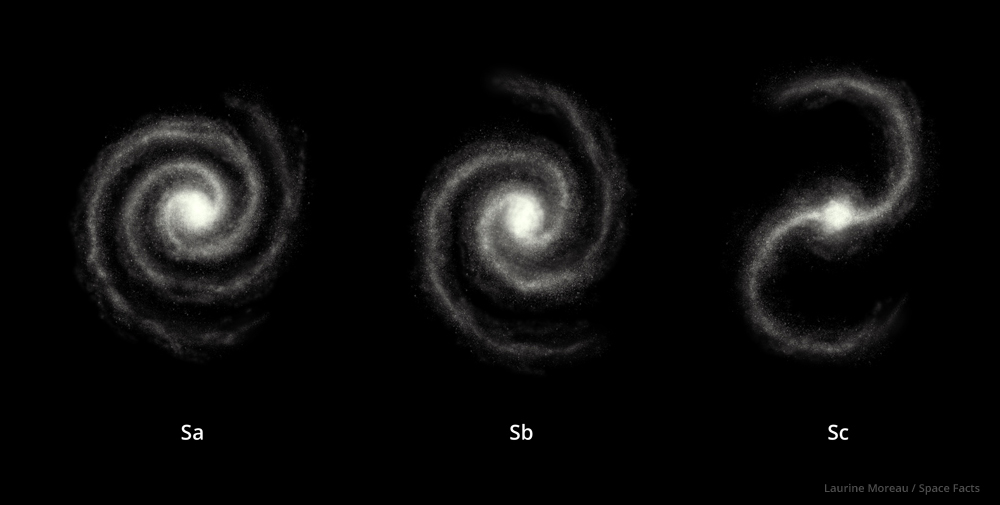
\includegraphics[scale=0.25]{galaxies/spiral/spiral-galaxies} \end{center}
			\end{itemize}
		\item $\frac{2}{3}$ spirals have an additional bar-like elongation of stars extending from the central bulge at the ends of which the spiral arms begin
			\begin{itemize}[noitemsep]
				\item the proportion of barred galaxies has changed over the history of the universe from 10\% to the current amt
				\item these are denoted by the additional label $SB$
				\begin{center} 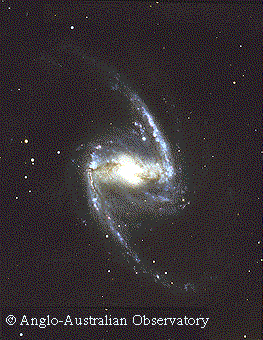
\includegraphics[scale=0.5]{galaxies/spiral/bar} \end{center}
			\end{itemize}
		\item \textbf{bulge} --- a huge, tightly packed central group of stars, often defined as the excess of stellar light above the inward extrapolation of the outer (exponential) disk light. Many bulges are thought to host a supermassive black hole at their centers.
	\end{itemize}
	\\
	\hline
	Celestial Bodies &
	\begin{itemize}[noitemsep]
\end{longtabu}
			